\subsection{WR PTP Core component}
\label{sec:hdl_wrpc}
This section describes the input and output ports of the WRPC IP-core and VHDL generic parameters
that can be used to personalize the core.

The top-level VHDL module is located under:\\\hrefwrpc{modules/wrc\_core/wr\_core.vhd}

A wrapper for the top-level VHDL module which makes use of VHDL records to reduce the number of
ports can be found under:\\\hrefwrpc{modules/wrc\_core/xwr\_core.vhd}

\begin{figure}
  \begin{center}
    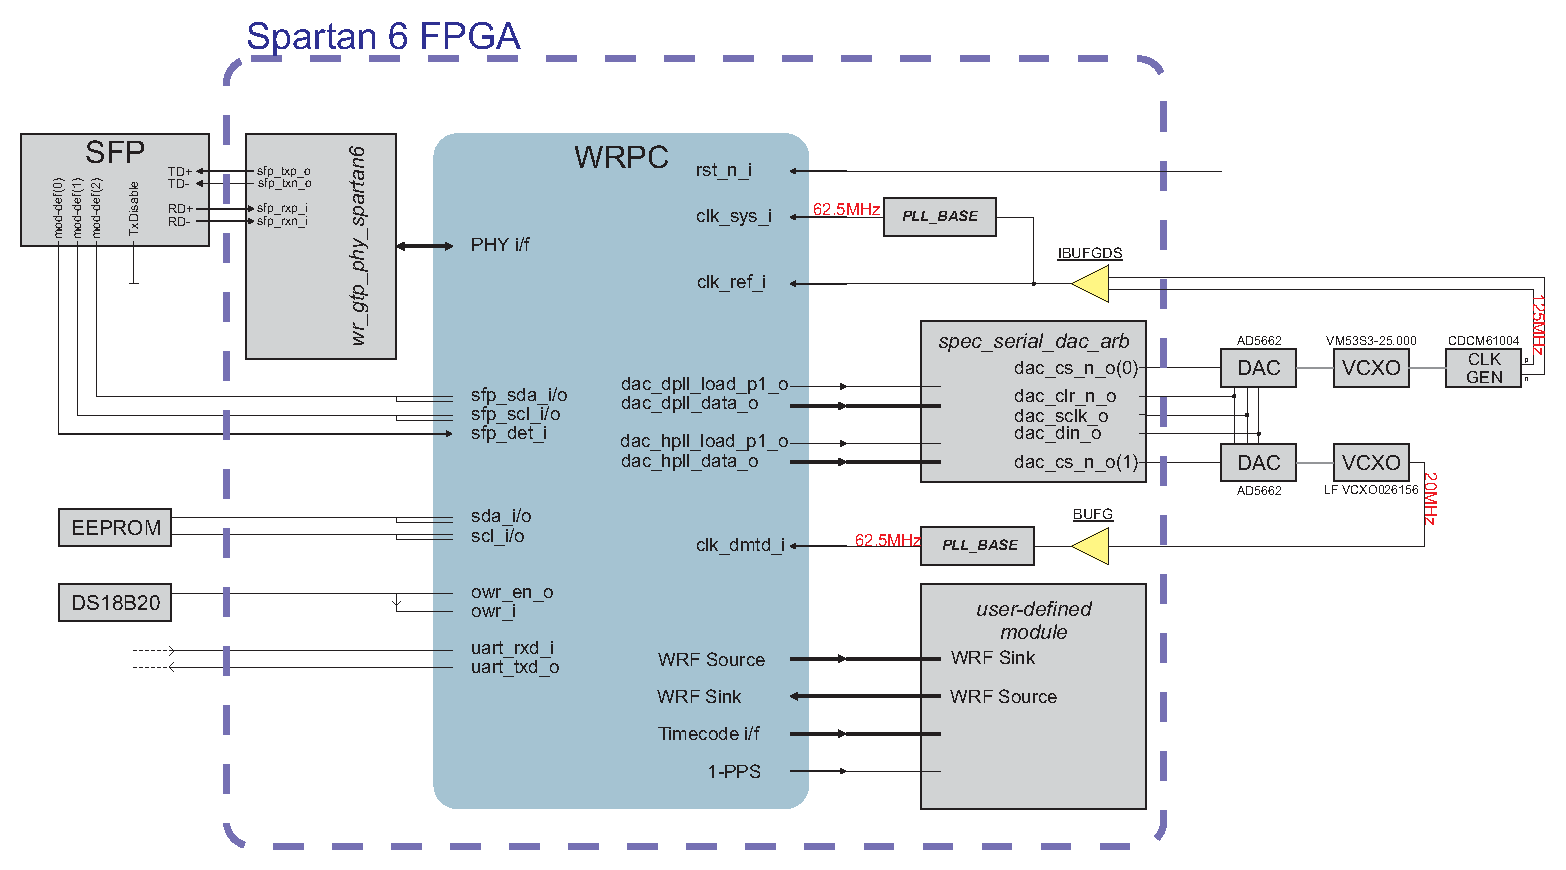
\includegraphics[width=.9\textheight, angle=270]{fig/basic_top.pdf}
    \caption{Simple top design with WRPC}
    \label{intro:fig:wrpc_top}
  \end{center}
\end{figure}

Figure \ref{intro:fig:wrpc_top} is an example on how to instantiate the WRPC component inside a
Xilinx Spartan6-based project. It contains few additional modules besides the WRPC:
\begin{itemize}
  \item \emph{wr\_gtp\_phy\_spartan6}: module wrapping Xilinx GTP SerDes to improve its determinism
  \item \emph{PLL\_BASE}: Xilinx Spartan6 PLL primitive \cite{pll_base}, used to produce 62.5 MHz
    system clock from 125 MHz local reference clock and to produce the DMTD offset clock from a
    local 20 MHz oscillator
  \item \emph{spec\_serial\_dac\_arb}: converts DACs tuning values to serial interface and
    arbitrates access to two DACs used for reference and DMTD clock tuning.
\end{itemize}

A very similar example can be found in the WRPC reference design for PCI-Express SPEC board (see
Section~\ref{sec:hdl_board_spec}).


\subsubsection{Generic parameters}
\label{sec:wrc_generics}

\begin{hdlparamtable}
  g\_simulation & integer & 0 & setting to '1' speeds up the simulation,
  must be set to '0' for synthesis\\
  \hline
  g\_with\_external\_clock\_input & boolean & false &
  enable external clock and 1-PPS inputs. The PLL inside WRPC will lock to
  external 10 MHz and 1-PPS signal when operating in GrandMaster mode\\
  g\_phys\_uart & boolean & true & enable physical UART interface\\
  \hline
  g\_virtual\_uart & boolean & false & enable virtual UART interface\\
  \hline
  g\_aux\_clks & integer & 0 & number of aux clocks syntonized by WRPC to WR timebase\\
  \hline
  g\_rx\_buffer\_size & integer & 1024 & size of Rx buffer in WRPC MAC module,
  default value is 1024 and should not be changed\\
  \hline
  g\_tx\_runt\_padding & boolean & true & when set to true, all user frames
  transmitted from the external fabric interface are padded if shorter than
  minimal Ethernet frame size (60B with header)\\
  \hline
  g\_dpram\_initf & string & "" & filename of compiled WRPC software, to be
  stored in WRPC memory during the synthesis (default is \emph{wrc.ram}
  created by compiling WRPC software from \emph{wrpc-sw} git repository)\\
  \hline
  g\_dpram\_size & integer & 32768 & size of RAM used by WRPC software (in 32-bit
  words), default value is 22528 and should not be changed\\
  \hline
  g\_interface\_mode & enum& PIPELINED & external Wishbone Slave interface mode
  \tts{[PIPELINED/CLASSIC]}\\
  \hline
  g\_address\_granularity & enum & BYTE & granularity of address bus in external
  Wishbone Slave interface \tts{[BYTE/WORD]}\\
  \hline
  g\_aux\_sdb & rec & c\_wrc\_periph3\_sdb & structure providing an SDB descriptor
  for the peripheral attached to the WRPC auxiliary WB interface. This parameter is optional
  and can be left unassigned. The default value corresponds to an undocumented device with an
  address space of 256 bytes\\
  \hline
  g\_softpll\_enable\_debugger & boolean & false & when set to true, additional
  FIFO is instantiated in the SoftPLL for collecting DMTD tags. It can be read
  out by the host and analyzed for SoftPLL debugging.\\
  \hline
  g\_vuart\_fifo\_size & integer & 1024 & size (in bytes) for the virtual UART FIFO\\
  \hline
  g\_pcs\_16bit & boolean & false & when set to \tts{true}, make use of 16-bit PCS, otherwise use 8-bit PCS\\
  \hline
  g\_records\_for\_phy & boolean & false & when set to \tts{true}, all the PHY-related
  signals will be grouped in the \tts{phy8/phy16} VHDL records, otherwise the individual standard
  logic signals will be used\\
  \hline
  g\_diag\_id  & integer & 0 & auxiliary diagnostics module ID\\
  \hline
  g\_diag\_ver & integer  & 0 & auxiliary diagnostics version for a given module ID\\
  \hline
  g\_diag\_ro\_size & integer & 0 & number of read-only registers fed to auxiliary diagnostics\\
  \hline
  g\_diag\_rw\_size & integer & 0 & number of read-write registers fed to
  auxiliary diagnostics\\  
\end{hdlparamtable}

\subsubsection{Ports}
\label{sec:wrc_ports}

\begin{hdlporttable}
  \hdltablesection{Clocks and resets}\\
  \hline
  clk\_sys\_i & in & 1 & main system clock, can be any frequency $\leq f_{clk\_ref\_i}$
  e.g. 62.5~MHz\\
  \hline
  clk\_dmtd\_i & in & 1 & DMTD offset clock (close to 62.5 MHz, e.g. 62.49 MHz)\\
  \hline
  clk\_ref\_i & in & 1 & 125 MHz reference clock\\
  \hline
  clk\_aux\_i & in & var & [optional] vector of auxiliary
  clocks that will be disciplined to WR timebase. Size is equal to \tts{g\_aux\_clks}\\
  \hline
  clk\_ext\_mul\_i & in & 1 & 125 MHz clock, derived from \tts{clk\_ext\_i}\\
  \hline
  clk\_ext\_mul\_locked\_i & in & 1 & PLL locked indicator for \tts{clk\_ext\_mul\_i}\\
  \hline
  clk\_ext\_stopped\_i & in & 1 & PLL stopped indicator for \tts{clk\_ext\_mul\_i}\\
  \hline
  clk\_ext\_rst\_o & out & 1 & Reset output to be used for \tts{clk\_ext\_mul\_i}\\
  \hline  
  clk\_ext\_i & in & 1 & [optional] external 10 MHz reference clock input for
  GrandMaster mode\\
  \hline
  pps\_ext\_i & in & 1 & [optional] external 1-PPS input used in GrandMaster mode\\
  \hline
  rst\_n\_i & in & 1 & main reset input, active-low (hold for at least 5
  \tts{clk\_sys\_i} cycles)\\
  \hline\pagebreak
  \hdltablesection{Timing system}\\
  \hline
  dac\_hpll\_load\_p1\_o & out & 1 & validates DAC value on data port \\
  \hline
  dac\_hpll\_data\_o & out & 16 & DAC value for tuning helper (DMTD) VCXO\\
  \hline
  dac\_dpll\_load\_p1\_o & out & 1 & validates DAC value on data port \\
  \hline
  dac\_dpll\_data\_o & out & 16 & DAC value for tuning main (ref) VCXO\\
  \hline
  \hdltablesection{PHY inteface (when \tts{g\_records\_for\_phy = false})}\\
  \hline
  phy\_ref\_clk\_i & in & 1 & TX clock\\
  \hline
  phy\_tx\_data\_o & out & var & TX data. If \tts{g\_pcs\_16bit = true}, then \tts{size = 16}, else \tts{size=8}\\
  \hline
  phy\_tx\_k\_o & out & var & \tts{1} when \tts{phy\_tx\_data\_o} contains a control code, \tts{0} when it's a data byte. If \tts{g\_pcs\_16bit = true}, then \tts{size = 2}, else \tts{size=1}\\
  \hline
  phy\_tx\_disparity\_i & in  & 1 & disparity of the currently transmitted 8b10b code (\tts{1} for positive, \tts{0} for negative)\\
  \hline
  phy\_tx\_enc\_err\_i & in  & 1 & TX encoding error indication\\
  \hline
  phy\_rx\_data\_i & in & var & RX data. If \tts{g\_pcs\_16bit = true}, then \tts{size = 16}, else \tts{size=8}\\
  \hline
  phy\_rx\_rbclk\_i & in & 1 & RX recovered clock\\
  \hline
  phy\_rx\_k\_i & in & var & \tts{1} when \tts{phy\_rx\_data\_i} contains a control code, \tts{0} when it's a data byte. If \tts{g\_pcs\_16bit = true}, then \tts{size = 2}, else \tts{size=1}\\
  \hline
  phy\_rx\_enc\_err\_i & in & 1 & RX encoding error indication\\
  \hline
  phy\_rx\_bitslide\_i & in & var & RX bitslide indication. If \tts{g\_pcs\_16bit = true}, then \tts{size = 5}, else \tts{size=4}\\
  \hline
  phy\_rst\_o & out & 1 & PHY reset, active high\\
  \hline
  phy\_rdy\_i & in & 1 & PHY is ready: locked and aligned\\
  \hline
  phy\_loopen\_o & out & 1 & \multirowpar{2}{local loopback enable (TX$\rightarrow$RX), active high}\\
  \cline{1-3}
  phy\_loopen\_vec\_o & out & 3 &\\
  \hline
  phy\_tx\_prbs\_sel\_o & out & 3 & PRBS select (see Xilinx UG386 Table 3-15; "000" = Standard operation, pattern generator off)\\
  \hline
  phy\_sfp\_tx\_fault\_i & in & 1 & SFP TX fault indicator\\
  \hline
  phy\_sfp\_los\_i & in & 1 & SFP Loss Of Signal indicator\\
  \hline
  phy\_sfp\_tx\_disable\_o & out & 1 & SFP TX disable control\\
  \hline
  \hdltablesection{PHY inteface (when \tts{g\_records\_for\_phy = true})}\\
  \hline
  phy8\_o & out & rec & \multirowpar{2}{input/output records for PHY signals
    when \tts{g\_pcs\_16bit = false}}\\
  \cline{1-3}
  phy8\_i & in & rec & \\
  \hline
  phy16\_o & out & rec & \multirowpar{2}{input/output records for PHY signals
    when \tts{g\_pcs\_16bit = true}}\\
  \cline{1-3}
  phy16\_i & in & rec & \\
  \hline\pagebreak
  \hdltablesection{GPIO}\\
  \hline
  led\_act\_o & out & 1 & signal for driving Ethernet activity LED\\
  \hline
  led\_link\_o & out & 1 & signal for driving Ethernet link LED\\
  \hline
  sda\_i & in  & 1 & \multirowpar{4}{I2C interface for EEPROM memory storing calibration}\\
  \cline{1-3}
  sda\_o & out & 1 & \\
  \cline{1-3}
  scl\_i & in  & 1 & \\
  \cline{1-3}
  scl\_o & out & 1 & \\
  \hline
  sfp\_sda\_i & in  & 1 & \multirowpar{4}{I2C interface for EEPROM inside SFP module}\\
  \cline{1-3}
  sfp\_sda\_o & out & 1 & \\
  \cline{1-3}
  sfp\_scl\_i & in  & 1 & \\
  \cline{1-3}
  sfp\_scl\_o & out & 1 & \\
  \hline
  sfp\_det\_i & in & 1 & SFP presence indicator\\
  \hline
  btn1\_i & in & 1 & \multirowpar{2}{two microswitch inputs, active low, currently not
    used in official WRPC software}\\
  \cline{1-3}
  btn2\_i & in & 1 & \\
  \hline
  spi\_sclk\_o & out & 1 & Flash SPI SCLK\\
  \hline
  spi\_ncs\_o  & out & 1 & Flash SPI $\overline{\mbox{SS}}$\\
  \hline
  spi\_mosi\_o & out & 1 & Flash SPI MOSI\\
  \hline
  spi\_miso\_i & in  & 1 & Flash SPI MISO\\
  \hline
  \hdltablesection{UART}\\
  \hline
  uart\_rxd\_i & in  & 1 & \multirowpar{2}{[optional] serial UART interface for
    interaction with WRPC software}\\
  \cline{1-3}
  uart\_txd\_o & out & 1 & \\
  \hline
  \hdltablesection{OneWire}\\
  \hline
  owr\_pwren\_o & out & 1 & \multirowpar{3}{[optional] 1-Wire interface used to read the
    temperature of hardware board from digital thermometer (e.g. Dallas DS18B20)}\\
  \cline{1-3}
  owr\_en\_o & out & 1 & \\
  \cline{1-3}
  owr\_i & in & 1 & \\
  \hline
  \hdltablesection{External WB interface}\\
  \hline
  wb\_adr\_i   & in & 32 & \multirowpar{11}{Wishbone slave interface that operates in
    Pipelined or Classic mode (selected with \tts{g\_interface\_mode}), with the address
    bus granularity controlled with \tts{g\_address\_granularity}}\\
  \cline{1-3}
  wb\_dat\_i   & in & 32 &\\
  \cline{1-3}
  wb\_dat\_o   & out & 32 &\\
  \cline{1-3}
  wb\_sel\_i   & in & 4 & \\
  \cline{1-3}
  wb\_we\_i    & in & 1 & \\
  \cline{1-3}
  wb\_cyc\_i   & in & 1 & \\
  \cline{1-3}
  wb\_stb\_i   & in & 1 & \\
  \cline{1-3}
  wb\_ack\_o   & out & 1 & \\
  \cline{1-3}
  wb\_err\_o   & out & 1 & \\
  \cline{1-3}
  wb\_rty\_o   & out & 1 & \\
  \cline{1-3}
  wb\_stall\_o & out & 1 & \\
  \hline
  wb\_slave\_o & out & rec & \multirowpar{2}{Alternative record-based ports
    for the WB slave interface (available in \tts{xwr\_core.vhd})}\\
  \cline{1-3}
  wb\_slave\_i & in & rec & \\
  \hline\pagebreak
  \hdltablesection{Auxiliary WB master}\\
  \hline
  aux\_adr\_i   & in & 32 & \multirowpar{11}{Auxilirary Wishbone pipelined
    master interface}\\
  \cline{1-3}
  aux\_dat\_o   & out & 32 &\\
  \cline{1-3}
  aux\_dat\_i   & in  & 32 &\\
  \cline{1-3}
  aux\_sel\_o   & out & 4 & \\
  \cline{1-3}
  aux\_we\_o    & out & 1 & \\
  \cline{1-3}
  aux\_cyc\_o   & out & 1 & \\
  \cline{1-3}
  aux\_stb\_o   & out & 1 & \\
  \cline{1-3}
  aux\_ack\_i   & in  & 1 & \\
  \cline{1-3}
  aux\_stall\_i & in  & 1 & \\
  \hline
  aux\_master\_o & out & rec & \multirowpar{2}{Alternative record-based
    ports for the aux WB master interface (available in \tts{xwr\_core.vhd})}\\
  \cline{1-3}
  aux\_master\_i & in & rec & \\
  \hline
  \hdltablesection{External fabric interface}\\
  \hline
  ext\_snk\_adr\_i & in & 2 & \multirowpar{9}{External fabric Wishbone
    pipelined interface, direction Sink$\rightarrow$Source}\\
  \cline{1-3}
  ext\_snk\_dat\_i & in & 16 & \\
  \cline{1-3}
  ext\_snk\_sel\_i & in & 2 & \\
  \cline{1-3}
  ext\_snk\_cyc\_i & in & 1 & \\
  \cline{1-3}
  ext\_snk\_stb\_i & in & 1 & \\
  \cline{1-3}
  ext\_snk\_we\_i  & in & 1 & \\
  \cline{1-3}
  ext\_snk\_ack\_o & out & 1 & \\
  \cline{1-3}
  ext\_snk\_err\_o & out & 1 & \\
  \cline{1-3}
  ext\_snk\_stall\_o & out & 1 & \\
  \hline
  ext\_src\_adr\_o & out & 2 & \multirowpar{9}{External fabric Wishbone
    pipelined interface, direction Source$\rightarrow$Sink}\\
  \cline{1-3}
  ext\_src\_dat\_o & out & 16 & \\
  \cline{1-3}
  ext\_src\_sel\_o & out & 2 & \\
  \cline{1-3}
  ext\_src\_cyc\_o & out & 1 & \\
  \cline{1-3}
  ext\_src\_stb\_o & out & 1 & \\
  \cline{1-3}
  ext\_src\_we\_o  & out & 1 & \\
  \cline{1-3}
  ext\_src\_ack\_i & in & 1 & \\
  \cline{1-3}
  ext\_src\_err\_i & in & 1 & \\
  \cline{1-3}
  ext\_src\_stall\_i & in & 1 & \\
  \hline
  wrf\_src\_o & out & rec & \multirowpar{4}{Alternative record-based
    ports for the fabric interface (available in \tts{xwr\_core.vhd})}\\
  \cline{1-3}
  wrf\_src\_i & in &  rec & \\
  \cline{1-3}
  wrf\_snk\_o & out & rec & \\
  \cline{1-3}
  wrf\_snk\_i & in &  rec & \\
  \hline\pagebreak
  \hdltablesection{External TX timestamp interface}\\
  \hline
  txtsu\_port\_id\_o & out & 5 & physical port ID from which the timestamp
  was originated. WRPC has only one physical port, so this value is always
  \tts{0}.\\
  \hline
  txtsu\_frame\_id\_o & out & 16 & frame ID for which the timestamp is
  available\\
  \hline
  txtsu\_ts\_value\_o & out & 32 & Tx timestamp value\\
  \hline
  txtsu\_ts\_incorrect\_o & out & 1 & Tx timestamp is not reliable since it
  was generated while PPS generator inside WRPC was being adjusted\\
  \hline
  txtsu\_stb\_o & out & 1 & strobe signal that validates the rest of signals
  described above\\
  \hline
  timestamps\_o & out & rec & Alternative record-based output ports for
  the TX timestamp interface (available in \tts{xwr\_core.vhd})\\
  \hline
  txtsu\_ack\_i & in & 1 & acknowledge, indicating that user-defined module
  has received the timestamp\\
  \hline
  \hdltablesection{Pause frame control}\\
  \hline
  fc\_tx\_pause\_req\_i   & in  &  1 & Ethernet flow control, request sending
  Pause frame\\
  \hline
  fc\_tx\_pause\_delay\_i & in  & 16 & Pause quanta\\
  \hline
  fc\_tx\_pause\_ready\_o & out &  1 & Pause acknowledge - active after the
  current pause send request has been completed\\
  \hline
  \hdltablesection{Timecode/Servo control}\\
  \hline
  tm\_link\_up\_o & out & 1 & state of Ethernet link (up/down), \tts{1}
  means Ethernet link is up\\
  \hline
  tm\_dac\_value\_o & out & 24 & DAC value for tuning auxiliary clock
  (\tts{clk\_aux\_i})\\
  \hline
  tm\_dac\_wr\_o & out & var & validates auxiliary DAC value. Size is equal
  to \tts{g\_aux\_clks}\\
  \hline
  tm\_clk\_aux\_lock\_en\_i & in & var & enable locking auxiliary clock to
  internal WR clock. Size is equal to \tts{g\_aux\_clks}\\
  \hline
  tm\_clk\_aux\_locked\_o & out & var & auxiliary clock locked to internal WR
  clock. Size is equal to \tts{g\_aux\_clks}\\
  \hline
  tm\_time\_valid\_o & out & 1 & if \tts{1}, the timecode generated by the
  WRPC is valid\\
  \hline
  tm\_tai\_o & out & 40 & TAI part of the timecode (full seconds)\\
  \hline
  tm\_cycles\_o & out & 28 & fractional part of each second represented by
  the state of counter clocked with the frequency 125 MHz (values from 0 to
  124999999, each count is 8 ns)\\
  \hline
  pps\_p\_o & out & 1 & 1-PPS signal generated in \tts{clk\_ref\_i} clock
  domain and aligned to WR time, pulse generated when the cycle counter is 0
  (beginning of each full TAI second)\\
  \hline
  pps\_led\_o & out & 1 & 1-PPS signal with extended pulse width to drive a LED\\
  \hline
  rst\_aux\_n\_o & out & 1 & Auxiliary reset output, active low\\  
  \hline
  link\_ok\_o & out & 1 & Link status indicator\\
  \hline
  \hdltablesection{Auxiliary diagnostics to/from external modules}\\
  \hline
  \linebreak aux\_diag\_i\linebreak & in & var & \multirowpar{2}{Arrays of
    32-bit vectors, to be accessed from WRPC via SNMP or uart console. Input array
    contains \tts{g\_diag\_ro\_size} elements, while output array contains
    \tts{g\_diag\_rw\_size} elements}\\
  \cline{1-3}
  \linebreak aux\_diag\_o\linebreak & out & var & \\
\end{hdlporttable}

\subsection{PHY interface}

\begin{figure}[ht]
  \begin{center}
    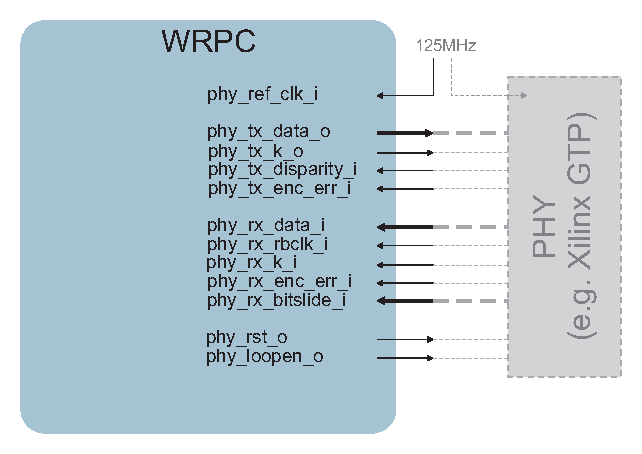
\includegraphics[width=.7\textwidth]{fig/wrpc_phyif.pdf}
    \caption{PHY interface of WRPC}
  \end{center}
\end{figure}

The interface connects WRPC with the Ethernet PHY layer IP-core. The interface is
generic, but currently two Gigabit Ethernet PHYs are tested and supported: Xilinx
8-bit GTP and 16-bit GTX SerDes. The signals' naming convention is the same as
in the GTP/GTX component definition.\\

{\bf Important !} If a WRPC user wants to use one of the supported PHYs (GTP,
GTX), they have to be taken from the White Rabbit HDL package instead of generating
them with the Xilinx Coregen tool. That is because WR developers have attached
additional logic to Xilinx GTP/GTX to improve its determinism.\\

\subsection{GPIO/UART/I2C/1-Wire/SPI interfaces}
\label{sec:wrpc_periph}

%\begin{figure}[ht]
%  \begin{center}
%    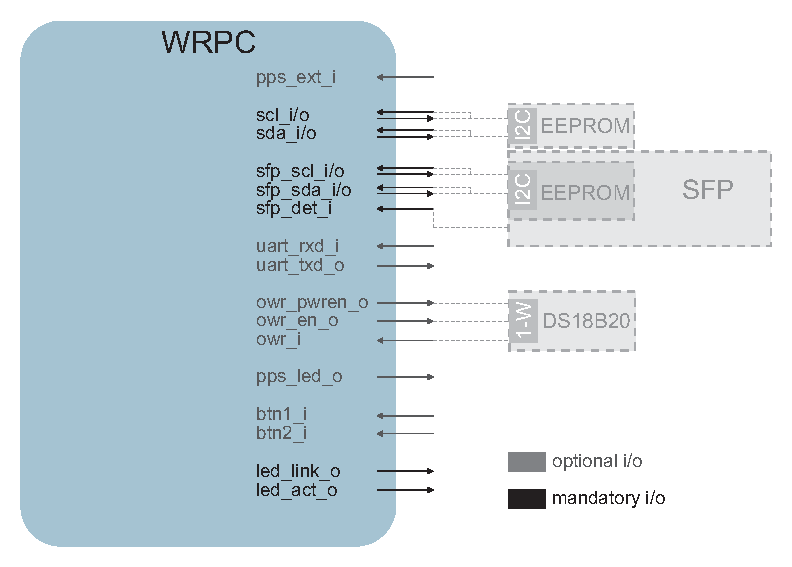
\includegraphics[width=.9\textwidth]{fig/basic_wrpc_gpio.pdf}
%    \caption{Other interfaces of WRPC}
%  \end{center}
%\end{figure}

Several hardware peripherals can be connected to the White Rabbit PTP Core. It
has:
\begin{itemize}
  \item UART - provides access to the WR PTP Core user shell
  \item 1-Wire - access to a digital thermometer for an on-board temperature and
    unique ID (used to generate a default MAC address of the WR port)
  \item SFP $I^2C$ - access to the SFP EEPROM, to read its ID and math with the
    calibration values
  \item SPI - access to the Flash memory, used to store calibration
    parameters and init script
  \item EEPROM $I^2C$ - [optional] access to the EEPROM memory, used to store
    calibration parameters and init script - currently SPI Flash is the
    preferred storage, however, EEPROM can still be used if needed.
\end{itemize}

\subsection{External Wishbone Slave/Master interface}

\begin{figure}[ht]
  \begin{center}
    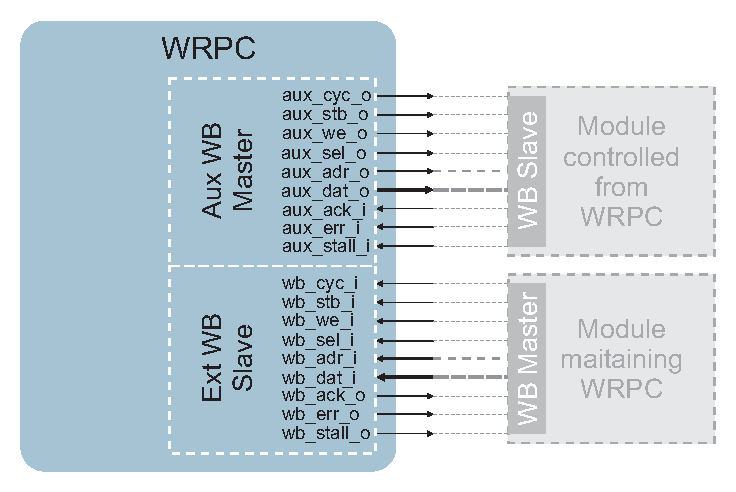
\includegraphics[width=.7\textwidth]{fig/wrpc_wb.pdf}
    \caption{External Wishbone interfaces of WRPC}
  \end{center}
\end{figure}

{\bf Aux WB Master} is a Pipelined Wishbone Master interface. It is connected
through the Wishbone Crossbar inside the White Rabbit PTP Core to the LM32 soft-core
processor (instantiated inside the WRPC). It can optionally be used to control
any user-defined module having a Pipelined Wishbone Slave interface. In that case, the WRPC software
has to be modified to control additional modules connected to the \emph{Aux WB
Master} interface.\\

{\bf Ext WB Slave} is a Wishbone Slave interface that operates in Pipelined or
Classic mode (selected with \emph{g\_interface\_mode} generic), with the address bus
granularity set with \linebreak \emph{g\_address\_granularity} generic. It gives the access
to control all the WRPC internals. In the WRPC reference design it is connected to
the Gennum GN4124 IP-core and used to upload WRPC software to its internal memory.\\

HDL modules accessible through \emph{Ext WB Slave} interface:
\begin{center}
  \begin{tabular}{|l|l|}
    \hline {\bf module name} & {\bf offset (bytes)}\\
    \hline
    WRPC internal memory & 0x00000\\
                Mini NIC & 0x20000\\
                Endpoint & 0x20100\\
                Soft PLL & 0x20200\\
           PPS generator & 0x20300\\
                  Syscon & 0x20400\\
                    UART & 0x20500\\
           1-Wire Master & 0x20600\\
           Aux WB Master & 0x20700\\
    \hline
  \end{tabular}
\end{center}

\subsubsection{Fabric interface}
\label{sec:wrpc_fabric}

The Fabric interface is used for sending and receiving Ethernet frames. It consists 
of two pipelined Wishbone interfaces operating independently: 

\begin{itemize}
  \item \emph{WRF Source}: pipelined Wishbone Master, passes all the Ethernet frames
    received from a physical link to WRF Sink interface implemented in a
    user-defined module.
  \item \emph{WRF Sink}: pipelined Wishbone Slave, receives Ethernet frames from
    the WRF Source implemented in the user-defined module, and sends them to a
    physical link.
\end{itemize}

{\bf Address bus} can have one of the following values:

\begin{center}
\begin{tabular}{|c|l|}
  \hline {\bf decimal value} & {\bf meaning of data word on data bus}\\
  \hline
  \emph{0} & regular data (packet header and payload)\\
  \emph{1} & OOB (Out-of-band) data\\
  \emph{2} & status word\\
  \emph{3} & currently not used\\
  \hline
\end{tabular}
\end{center}

{\bf Status word} (sent when the value of address bus is \emph{2}) contains
various information about Ethernet frame's structure and type:
%\begin{figure}[ht]
  \begin{center}
    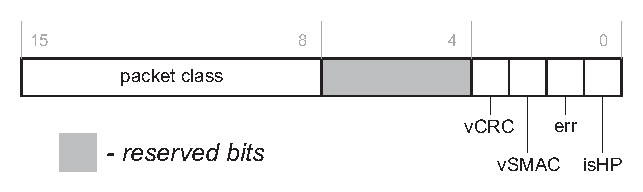
\includegraphics[width=.6\textwidth]{fig/status.pdf}
    %\caption{Status word format}
  \end{center}
%\end{figure}

\begin{itemize}
  \item[] \emph{isHP} - if \emph{1}, the frame is high priority
  \item[] \emph{err} - if \emph{1}, the frame contains an error
  \item[] \emph{vSMAC} - the frame contains a source MAC address (otherwise
    it will be assigned from WRPC configuration)
  \item[] \emph{vCRC} - the frame contains a valid CRC checksum
  \item[] \emph{packet class} - the packet class assigned by the classifier
    inside WRPC MAC module
\end{itemize}

OOB data is used for passing the timestamp-related information for the incoming and 
outgoing Ethernet frames. Each frame received from a physical link is
timestamped inside the WRPC and this value is passed as Rx OOB
data. On the other hand, for each transmitted frame the Tx timestamp can be read
from the Tx Timestamping Interface (section \ref{sec:txts}) together with a unique
frame number assigned in Tx OOB. Therefore, the format of OOB differs between Rx
and Tx frames.\\

{\bf Tx OOB format}:

%\begin{figure}[ht]
  \begin{center}
    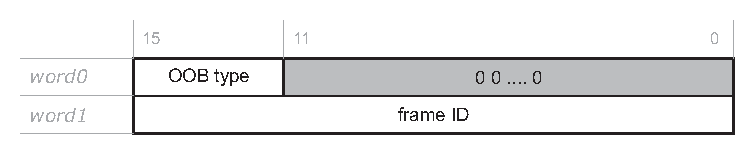
\includegraphics[width=.7\textwidth]{fig/oob_tx.pdf}
    %\caption{Tx OOB data format}
    %\label{fig:fabric_adv:tx_oob}
  \end{center}
%\end{figure}

\begin{itemize}
  \item[] \emph{OOB type}: "0001" means Tx OOB
  \item[] \emph{frame ID}: ID of the frame being sent. It is later output
    through the \emph{Tx Timestamping interface} to associate Tx timestamp with
    appropriate frame. Frame ID = 0 is reserved for PTP packets inside WRPC
    and cannot be used by user-defined modules.
\end{itemize}

{\bf Rx OOB format}:
%\begin{figure}[ht]
  \begin{center}
    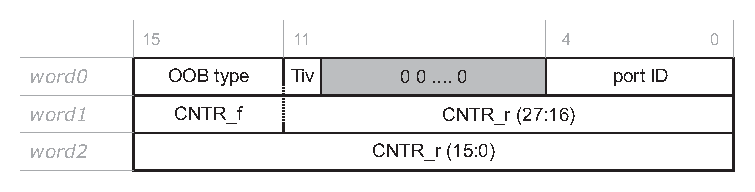
\includegraphics[width=.7\textwidth]{fig/oob_rx.pdf}
    %\caption{Rx OOB data format}
    %\label{fig:fabric_adv:rx_oob}
  \end{center}
%\end{figure}

\begin{itemize}
  \item[] \emph{OOB type}: "0000" means Rx OOB
  \item[] \emph{Tiv}: timestamp invalid. When this bit is set to '1', the PPS
    generator inside WRPC is being adjusted which means the Rx timestamp is not
    reliable.
  \item[] \emph{port ID}: the ID of a physical port on which the packet was
    received. In case of WRPC, this field is always 0, because there is only one
    physical port available.
  \item[] \emph{CNTR\_f}: least significant bits of the Rx timestamp generated on
    the falling edge of the reference clock.
  \item[] \emph{CNTR\_r}: Rx timestamp generated on the rising edge of the reference
    clock.
\end{itemize}

\begin{figure}
  \begin{center}
    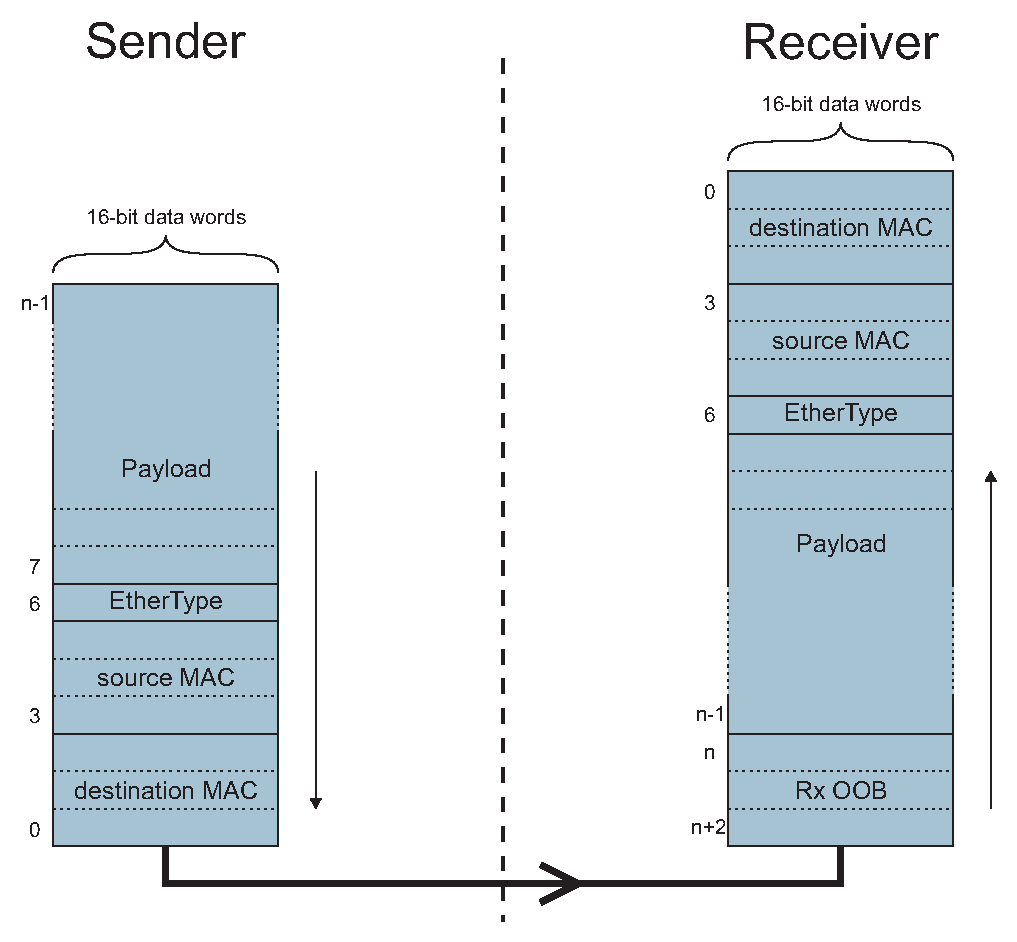
\includegraphics[width=.6\textwidth]{fig/basic_wrf_data.pdf}
    \caption{Data words that make the Ethernet frame}
    \label{fig:fabric:simple_data}
  \end{center}
\end{figure}

Figure \ref{fig:fabric:simple_data} presents data words fed to the WRF
data bus by the sender and the information got at the receiving side. Please
note that the CRC checksum is calculated and inserted automatically inside the
WRPC and user-defined module doesn't care about it. The Ethernet frame received
from the WR Fabric interface may contain additional OOB data suffixed. It has to
be received (acknowledged) by the user-defined module, but can be simply discarded.

\newparagraph{Examples}
Figure \ref{fig:fabric:simple_tx} shows a very simple WR Fabric cycle. The WRF
Source of user-defined module sends there an Ethernet frame containing even
number of bytes.

\begin{figure}
  \begin{center}
    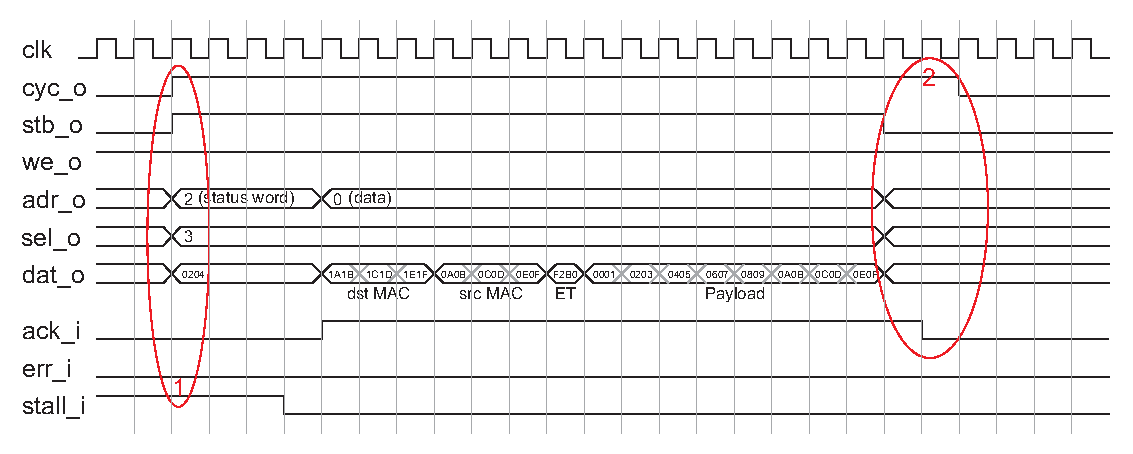
\includegraphics[width=\textwidth]{fig/basic_wrf_cycle_simple.pdf}
    \caption{Simple WR Fabric cycle - user-defined module sending packet}
    \label{fig:fabric:simple_tx}
  \end{center}
\end{figure}

\begin{enumerate}
  \item The WRF Source in user-defined module starts the cycle by asserting
    \emph{cyc\_o}, \emph{stb\_o} and putting a status word to the data bus.
    However, since WRF Sink set \emph{stall} signal to active state, Source has
    to wait until Sink is ready to receive data.
  \item After the last word is transmitted, the WRF Source sets \emph{stb\_o} back
    to \emph{0}, but waits until Sink acknowledges all the words transmitted in
    the cycle (\emph{ack\_i} line). The cycle ends when \emph{cyc\_o} goes back
    to the low state.
\end{enumerate}

Figure \ref{fig:fabric:sel} shows again a very simple WR Fabric cycle where
user-defined WRF Source sends an Ethernet frame to the WRPC. This time though,
the frame contains odd number of bytes, therefore the \emph{sel} line is used to
signal this fact to WRF Sink inside the WRPC (1).

\begin{figure}
  \begin{center}
    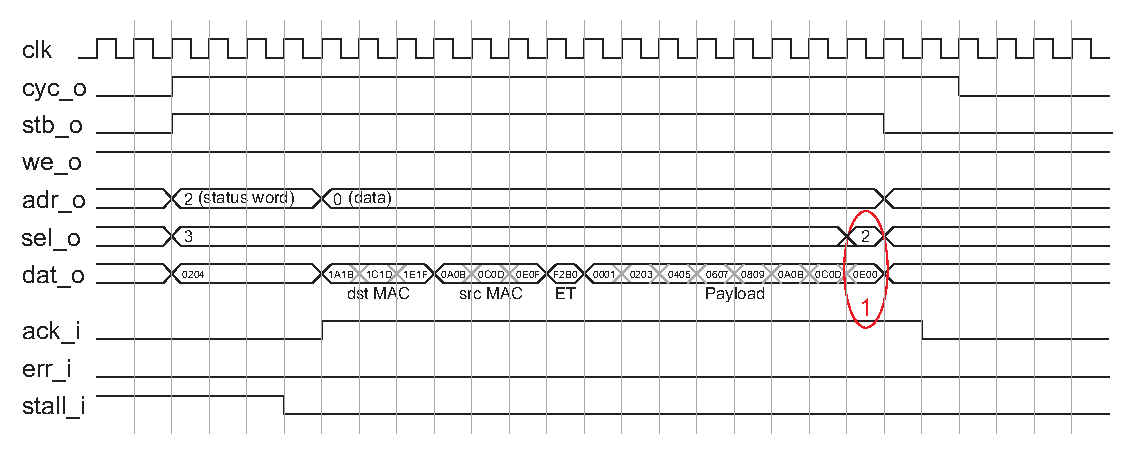
\includegraphics[width=\textwidth]{fig/basic_wrf_cycle_sel.pdf}
    \caption{Simple WR Fabric cycle - user-defined module sending packet(odd
    number of bytes in the payload)}
    \label{fig:fabric:sel}
  \end{center}
\end{figure}

Figure \ref{fig:fabric:cyc} presents more complicated Fabric cycle where an
Ethernet frame is received from WRF Source in the WRPC (output signals in the
diagram are driven by WRF Source on the WRPC side): 

\begin{figure}
  \begin{center}
    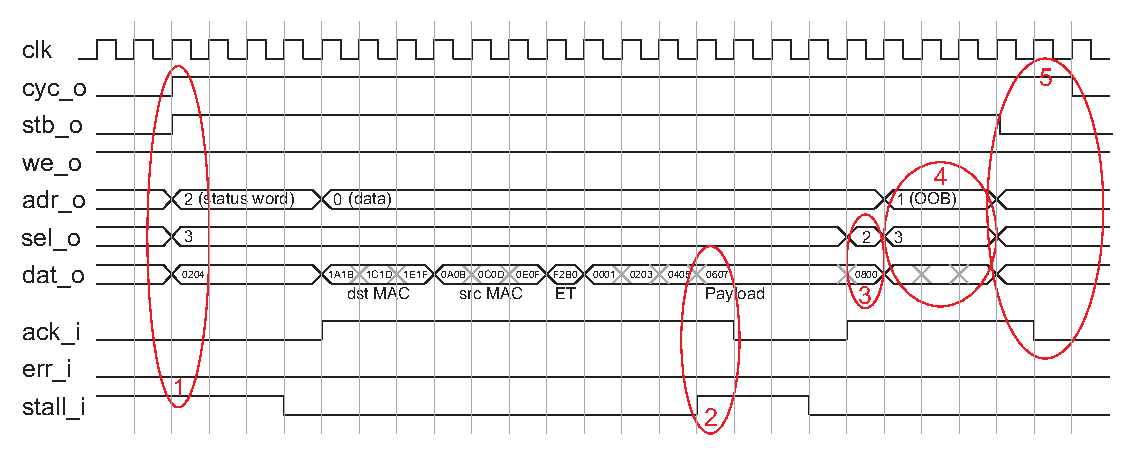
\includegraphics[width=\textwidth]{fig/basic_wrf_cycle.pdf}
    \caption{WR Fabric cycle}
    \label{fig:fabric:cyc}
  \end{center}
\end{figure}
\begin{enumerate}
  \item The WRF Source starts the cycle by asserting \emph{cyc\_o}, \emph{stb\_o}
    and putting a status word to the data bus. However, since WRF Sink set 
    \emph{stall} signal to active state, Source has to wait until Sink is ready
    to receive data.
  \item While the payload of the Ethernet frame is being transmitted, Sink
    stalls the cycle. The WRF Source pauses the transmission until Sink becomes
    ready to process the rest of the data. During that time \emph{stb\_o} has to
    remain in a high state.
  \item The Ethernet frame contains an odd number of bytes, so only half of last
    word of payload carries a valid data. \emph{Sel\_o} is used to signal this
    fact to WRF Sink.
  \item After the whole payload is transmitted, Source may additionally sent Rx
    OOB data. It contains some internal WRPC data that should be acknowledged
    by Sink, but discarded in the user's module.
  \item After the last word is transmitted, the WRF Source sets \emph{stb\_o} back
    to \emph{0}, but waits until Sink acknowledges all the words transmitted in
    the cycle (\emph{ack\_i} line). The cycle ends when \emph{cyc\_o} goes back
    to the low state.
\end{enumerate}

WRF Sink can use the \emph{stall} line to pause the frame transmission if it cannot
process the flow of data coming from WRF Source. However, if some more serious
problem appears on the receiving side, the \emph{err} line can be used to
immediately break the cycle. This situation is presented in figure
\ref{fig:fabric:cycerr}:

\begin{figure}
  \begin{center}
    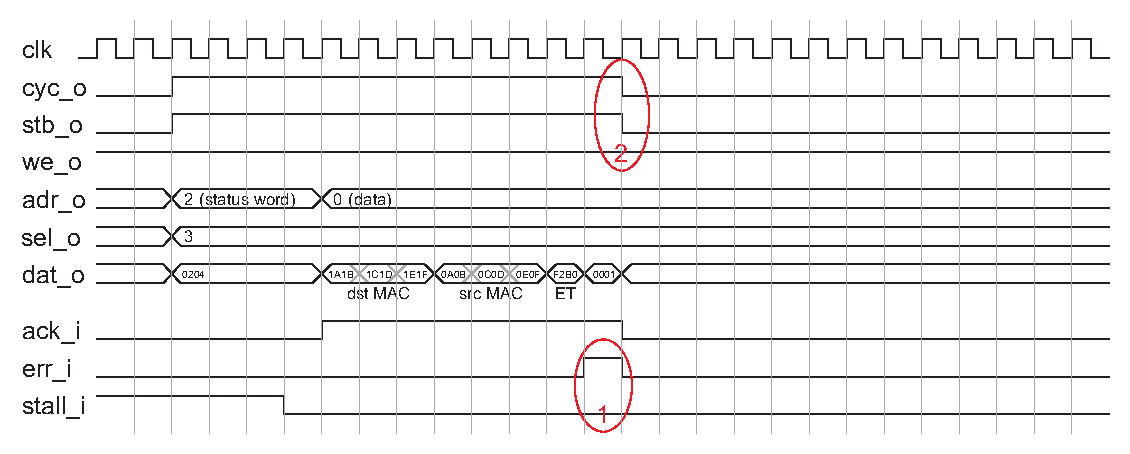
\includegraphics[width=\textwidth]{fig/basic_wrf_cycle_err.pdf}
    \caption{WR Fabric cycle interrupted with an error line}
    \label{fig:fabric:cycerr}
  \end{center}
\end{figure}

\begin{enumerate}
  \item WRF Sink wants to break a bus cycle, so it drives \emph{err\_i} high.
  \item WRF Source breaks the cycle immediately after receiving an error indicator
    from the WRF Sink.
\end{enumerate}

\newparagraph{SystemVerilog model}
The SystemVerilog simulation model of the WR Fabric interface (both WRF Source and 
WRF Sink) can be found in the \emph{wr-cores} git repository
(git://ohwr.org/hdl-core-lib/wr-cores.git) and consists of the files:
\begin{itemize}
  \item \emph{sim/if\_wb\_master.svh}
  \item \emph{sim/if\_wb\_slave.svh}
  \item \emph{sim/wb\_packet\_source.svh}
  \item \emph{sim/wb\_packet\_sink.svh}
\end{itemize}

The testbench example using the simulation model of WR Fabric interface can
be found in the zip archive attached to this documentation.


\subsubsection{Tx Timestamping interface}
\label{sec:txts}

The Tx Timestamping interface provides the timestamps generated inside WRPC for each
Ethernet frame transmitted from user-defined module through the WRF Sink interface.\\


\subsubsection{Timecode interface}
\label{sec:wrpc_timecode}

%\begin{figure}[ht]
%  \begin{center}
%    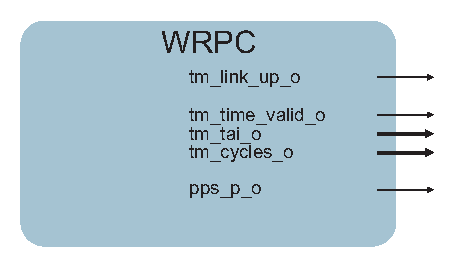
\includegraphics[width=.5\textwidth]{fig/basic_wrpc_tm.pdf}
%    \caption{Timecode output interface of WRPC}
%  \end{center}
%\end{figure}

Timecode interface provides current time to the other HDL modules in a form that
can be easily used. It consists of: a 1-PPS and a UTC timecode
aligned to the time of WR Master.


\subsection{Auxiliary diagnostics interface}
\label{sec:aux_diag}

Auxiliary diagnostics interface can be used if a user would like to benefit from
the WR PTP Core diagnostics capabilities to export some registers from his/her
IP core. The interface consists of two 32-bit \texttt{std\_logic\_vector}
arrays. User-defined registers that are to be read from the WRPC SNMP agent (SNMP
GET requests), should be connected to the \texttt{aux\_diag\_i} vector.
User-defined values that are written from the WRPC SNMP agent (SNMP SET
requests) will be available in the \texttt{aux\_diag\_o} vector.

Two VHDL generics \texttt{g\_diag\_id} and \texttt{g\_diag\_ver} are used to let
the user uniquely identify given application (user-defined set of registers)
to match it with appropriate, custom SNMP MIB file.

